
\chapter{Robot-Camera Calibration}
\label{chap:robot}
This section presents the theory as well as each individual step for estimating the pose of the camera relative to the robot base frame, the problem to be solved is an extrinsic camera calibration (also known as a robot-camera calibration or Eye-to-hand calibration), but an intrinsic camera calibration needs to be solved a priori. The robot-camera calibration is a fundamental part of the subsequent use in the next chapter of this thesis. The extrinsic camera calibration methods generally require the position of the camera frame relative to a calibration target frame to be known. Therefore, the proposed method to solve the robot-camera calibration task for this thesis is based on tracking a calibration target (standard checkerboard calibration grid) attached to the end-effector of the robot with known forward kinematics. 


\section{Camera Calibration}

Camera calibration is the process of estimating intrinsic and extrinsic parameters. The intrinsic parameters deal with the camera's internal characteristics, such as its focal distance, distortion, and image centre. The extrinsic parameters represent the position and orientation relative to the calibration target. In this thesis the camera calibration is treated separately and can be divided into two main stages:

\begin{itemize}
\item Sensor internal parameter calibration, like lens distortion, focal distance, optical center (image center) described above. In addiction to that, for RGB-D cameras, color and depth image offsets.
\item Robot-camera calibration: the pose(position and orientation) of a camera coordinate system in a reference coordinate frame. In this thesis we also refer as to Eye-to-Hand calibration. The transformation from the camera coordinate system to the robot base coordinates system (also called world coordinates system interchangeably in this thesis) is shown in Figure\ref{fig:system0} 

\end{itemize}
\begin{figure}[!h]
\begin{center}
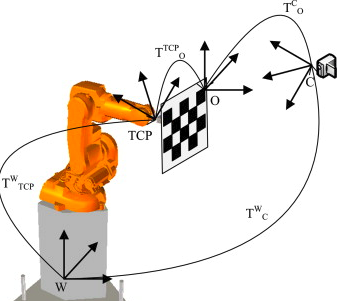
\includegraphics[width=3in]{figures03/system1.png}
\caption{Overview of the camera pose estimation system. The system estimates  the pose of the camera frame relative to the world frame(also known as robot base frame). Image from \cite{autCAL}.}
\label{fig:system0}
\end{center}
\end{figure}

Normally, it is sufficient to perform an internal camera parameter calibration only once for each device unless the lens or sensors itself will be changed or modified. Reliable calibration methods already exist, which are widely used \cite{Zhang} \cite{Tsai}.

Robot-camera calibration, on the other hand, is more application specific and an important stage of any 6-DoF pose estimation system. 

\section{Sensor internal parameter calibration}

\subsection{Camera Model} \label{intrinsic}

The choice of camera model influences the final calibration results, so the first step is to select an appropriate camera model. In this thesis, the pinhole camera model \ref{pinhole} is used. It describes the mathematical relationship between the coordinates of a point in three-dimensional space and its projection onto the image plane of an ideal camera. 

The MATLAB, Open CV  and the $camera\textunderscore calibration$ ROS  \cite{calRos} packages are the most popular systems for camera calibration. They are already available for checkerboard detection based on the pinhole model and the method proposed by Zhang \cite{Zhang}, All of them introduce the radial distortion and tangential distortion. In this thesis, the OpenCV and $camera\textunderscore calibration$ ROS packages are used for the purpose of comparison in this thesis.
The technique proposed by Zhang only requires the camera to observe a calibration target shown at few (at least three) different orientations. the technique relates known points in the world to points in an image, in order to do so, one must first acquire a series of known world points. The most common method is to use known planar objects(checkerboard calibration grid) at different orientations with respect to the camera to develop an independent series of data points. The calibration object chosen in this thesis is a 6x9 checkerboard with the corner points as the known world points and it can be seen in Figure \ref{fig:target0}.

\begin{figure}[!h]
\begin{center}
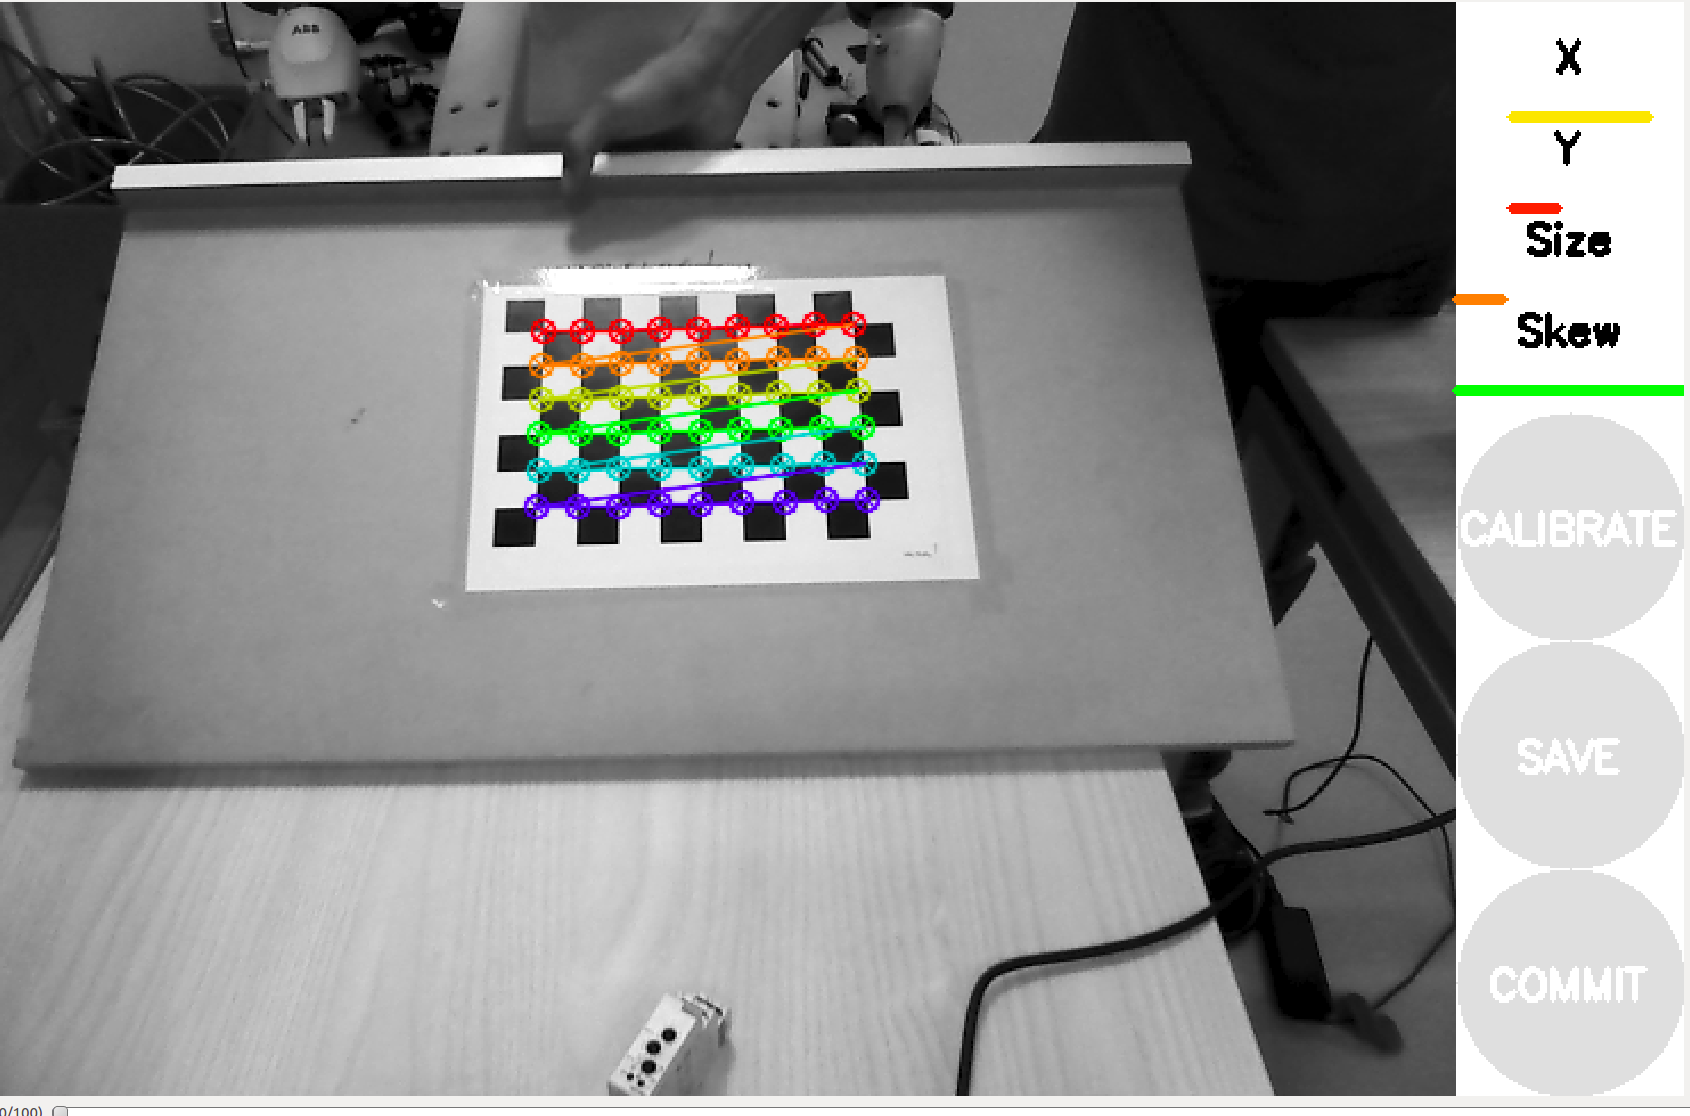
\includegraphics[width=3in]{figures03/intros.png}
\caption{Overview of the intrinsic calibration based on industrial calibration ROS package with a 6X9 checkerboard calibration target}%\cite{temp2}}
\label{fig:target0}
\end{center}
\end{figure}

\section{Eye-to-Hand Calibration}

In order to know the pose of the camera coordinate system relative to the world coordinate system also known as robot base frame, extrinsic calibration (estimation of the rotation and translation of the camera frame) methods will be used. In this thesis, the method for extrinsic camera calibration based on calibration planer target is used. It is assumed camera intrinsic parameters and distortion coefficients are known a priori as describe in \ref{intrinsic} and fixed during the entire sequence. Such a system is shown in Figure \ref{fig:camposest}.

\begin{figure}[!h]
\begin{center}
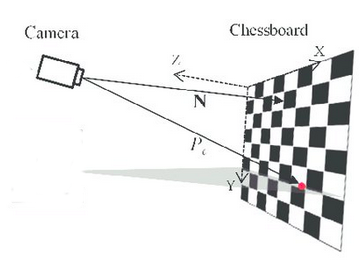
\includegraphics[width=3in]{figures03/camposest.png}
\caption{Overview of the camera pose estimation system. The system estimates the distance
and orientation to the local coordinate system of the checkerboard}%\cite{temp2}}
\label{fig:camposest}
\end{center}
\end{figure}

\subsection{Calibration Targets}
There are many types of camera calibration targets for use in imaging systems. In this thesis the planar targets are use since they can be easily printed with a standard
printer and fixed to a surface. Planar targets can be subdivided as follow:
\begin{itemize}
\item Repeated pattern e.g. checkerboard patterns 
\item Non repeated pattern e.g augmented Reality (AR)
\end{itemize}

\subsection{Checkerboard Patterns}

Checkerboard calibration targets are one of the most frequently-used targets, where the calibration points are the corner points between squares. This pattern is simple to produce and allows for high accuracy because the corner points can be detected to subpixel precision. For example, the popular OpenCV library already contains algorithms to automatically locate plain checkerboards. Figure \ref{fig:target1} shows an example of checkerboard calibration target.


\begin{figure}[!h]
\begin{center}
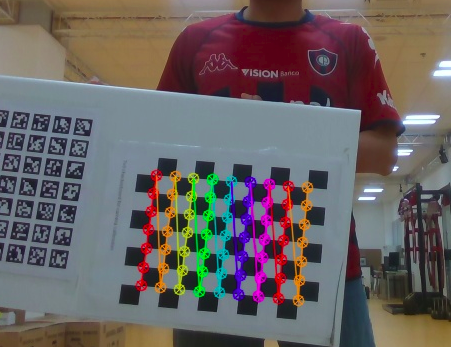
\includegraphics[width=3in]{figures03/openCV1.png}
\caption{Overview of a 7X9 checkerboard calibration grid }%\cite{temp2}}
\label{fig:target1}
\end{center}
\end{figure}

\subsection{Augmented Reality (AR)}
AR markers also called Fiducial (individually identifiable) markers have become increasingly popular in recent years. Such markers can be used in a variety of settings such as camera calibration, where small markers are used, those who encode a unique code for identification purposes. There are a large number of markers available. One of the most common fiducial marker designs includes rectangular patterns with identification codes in the interior such as $ARTag (2005)$, AprilTag and CALTag to name few of them.  Refer to \cite{fiducialTargets} 


\begin{figure}[!h]
\begin{center}
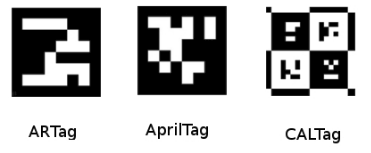
\includegraphics[width=3in]{figures03/fiducials.png}
\caption{ARTag, AprilTag and CALTag markers example. Image from \cite{fiducialTargets}}%\cite{temp2}}
\label{fig:fiducial}
\end{center}
\end{figure}

\subsection{Selection}
In this thesis, the checkerboard pattern is used.  This pattern is simple to produce and allows for high accuracy because the corner points can be detected to subpixel precision \cite{planarTargets}.







\begin{figure}[!h]
\begin{center}
\includegraphics[width=4in]{figures03/setup.png}
\caption{Overview of the setup, a ABB YUMI robot with a gripper holding the calibration plate. The camera is fixed around the robot workspace and pointed at the checkerboard}%\cite{temp2}}
\label{fig:setup}
\end{center}
\end{figure}



\iffalse




\begin{figure}[!h]
\begin{center}
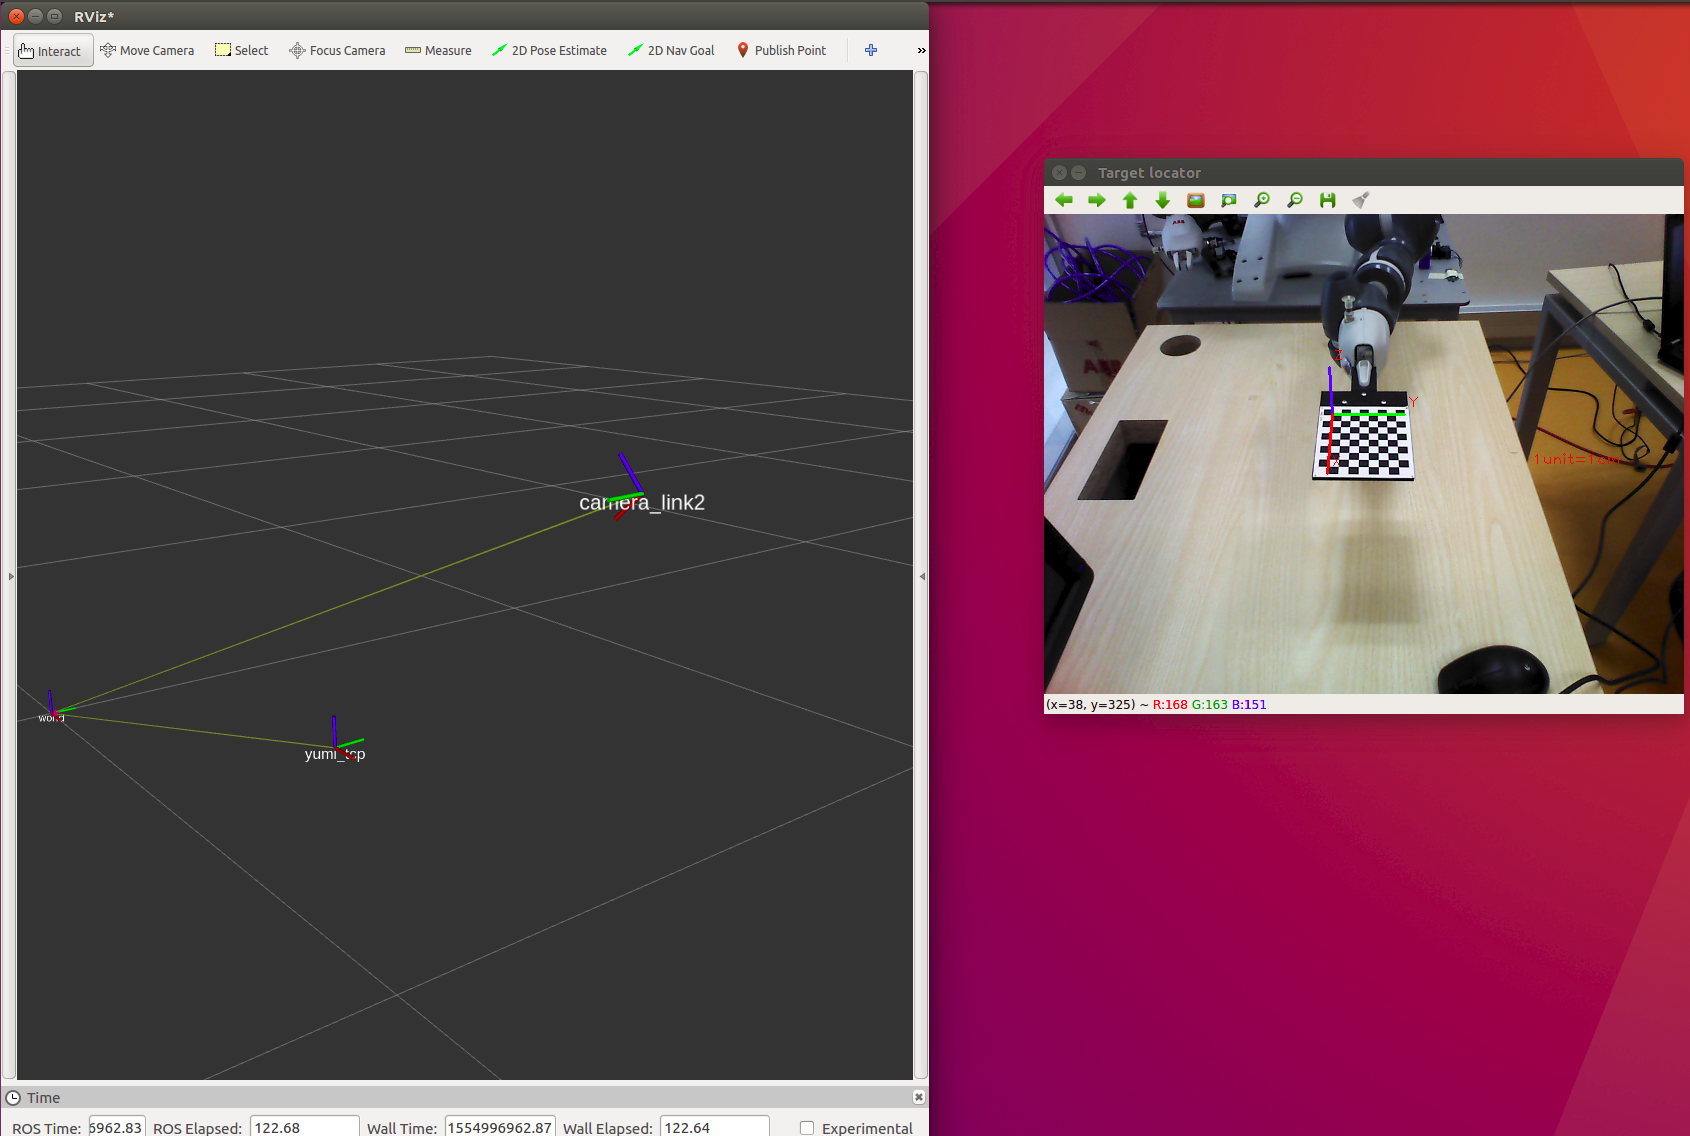
\includegraphics[width=3in]{figures03/rviz1.png}
\caption{Overview of the intrinsic calibration based on industrial calibration (ROS package)}%\cite{temp2}}
\label{fig:rosCAL}
\end{center}
\end{figure}



\begin{figure}[!h]
\begin{center}
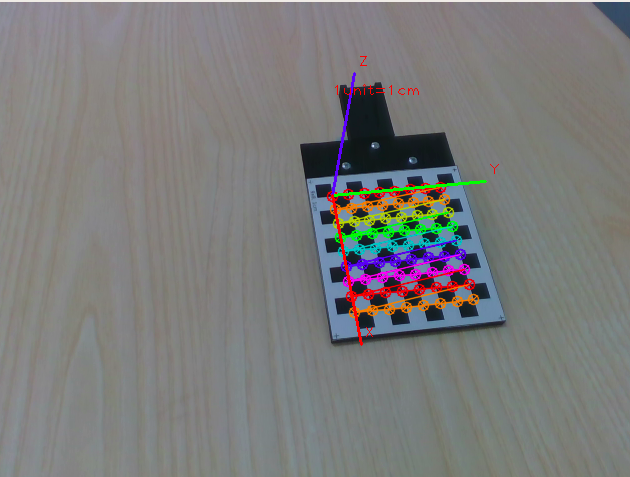
\includegraphics[width=3in]{figures03/calibrationtarget1.png}
\caption{Checkerboard Calibration Target}%\cite{temp2}}
\label{fig:pipeline}
\end{center}
\end{figure}

Camera calibration procedure is performed to obtain the intrinsic and extrinsic camera parameters.The intrinsic parameters are used for obtaining the relative position of the object according to the frame fixed with camera. This procedure is performed only once. The extrinsic parameters are the pose (translation and rotation) of the camera frame with respect to the robot-base frame, this procedure needs to be repeated each time the position of the camera changed with respect to the robot-base frame. 


The robot-camera calibration is based on a checkerboard calibration target attached rigidly to the end-effector of the robot. The position of the calibration target in the end-effector frame is estimated according to the design of the calibration plate in the FreeCAD software, and the pose between the camera frame and the robot base frame is calculated by the Eq. , for convinience of faster calculation, we use the tf-ROS package. The overview of the estimated parameters is presented in Figure. \ref{fig:rviz1} 



industrial calibration OpenCV 2.3 library are used. For cameras position calibration,method presented by Motai and Kosaka[13]has been adopted andimplemented
Although not being the main focus of this project, robot-camera calibration is an essential part for the subsequent step, recognition and estimation of the position of an object with a camera, the main objective of this master thesis. Therefore, the exact transformation between the base frame of the robot and the camera has to be known. 

\fi




































